\documentclass[]{book}
\usepackage{lmodern}
\usepackage{amssymb,amsmath}
\usepackage{ifxetex,ifluatex}
\usepackage{fixltx2e} % provides \textsubscript
\ifnum 0\ifxetex 1\fi\ifluatex 1\fi=0 % if pdftex
  \usepackage[T1]{fontenc}
  \usepackage[utf8]{inputenc}
\else % if luatex or xelatex
  \ifxetex
    \usepackage{mathspec}
  \else
    \usepackage{fontspec}
  \fi
  \defaultfontfeatures{Ligatures=TeX,Scale=MatchLowercase}
\fi
% use upquote if available, for straight quotes in verbatim environments
\IfFileExists{upquote.sty}{\usepackage{upquote}}{}
% use microtype if available
\IfFileExists{microtype.sty}{%
\usepackage{microtype}
\UseMicrotypeSet[protrusion]{basicmath} % disable protrusion for tt fonts
}{}
\usepackage{hyperref}
\hypersetup{unicode=true,
            pdfborder={0 0 0},
            breaklinks=true}
\urlstyle{same}  % don't use monospace font for urls
\usepackage{longtable,booktabs}
\usepackage{graphicx,grffile}
\makeatletter
\def\maxwidth{\ifdim\Gin@nat@width>\linewidth\linewidth\else\Gin@nat@width\fi}
\def\maxheight{\ifdim\Gin@nat@height>\textheight\textheight\else\Gin@nat@height\fi}
\makeatother
% Scale images if necessary, so that they will not overflow the page
% margins by default, and it is still possible to overwrite the defaults
% using explicit options in \includegraphics[width, height, ...]{}
\setkeys{Gin}{width=\maxwidth,height=\maxheight,keepaspectratio}
\IfFileExists{parskip.sty}{%
\usepackage{parskip}
}{% else
\setlength{\parindent}{0pt}
\setlength{\parskip}{6pt plus 2pt minus 1pt}
}
\setlength{\emergencystretch}{3em}  % prevent overfull lines
\providecommand{\tightlist}{%
  \setlength{\itemsep}{0pt}\setlength{\parskip}{0pt}}
\setcounter{secnumdepth}{5}
% Redefines (sub)paragraphs to behave more like sections
\ifx\paragraph\undefined\else
\let\oldparagraph\paragraph
\renewcommand{\paragraph}[1]{\oldparagraph{#1}\mbox{}}
\fi
\ifx\subparagraph\undefined\else
\let\oldsubparagraph\subparagraph
\renewcommand{\subparagraph}[1]{\oldsubparagraph{#1}\mbox{}}
\fi

%%% Use protect on footnotes to avoid problems with footnotes in titles
\let\rmarkdownfootnote\footnote%
\def\footnote{\protect\rmarkdownfootnote}

%%% Change title format to be more compact
\usepackage{titling}

% Create subtitle command for use in maketitle
\providecommand{\subtitle}[1]{
  \posttitle{
    \begin{center}\large#1\end{center}
    }
}

\setlength{\droptitle}{-2em}

  \title{}
    \pretitle{\vspace{\droptitle}}
  \posttitle{}
    \author{}
    \preauthor{}\postauthor{}
    \date{}
    \predate{}\postdate{}
  
% Starts each section (##) on a new page
% https://tex.stackexchange.com/questions/9497/start-new-page-with-each-section
\let\stdsection\section
\renewcommand\section{\clearpage\stdsection}

% Needs latex_engine: xelatex in _output.yml. Doesn't work yet.
\usepackage{fontspec}

\begin{document}

%\newgeometry{tmargin=1.5cm,lmargin=2.5cm,rmargin=2.5cm,bmargin=0.5cm} %verbose

\begin{titlepage}
\begin{center}
  

\end{center}
\vspace{1.5cm}
\begin{center}

{\LARGE Songs}

\end{center}
 \vspace{1cm}

\begin{figure}[htbp]
  \centering
  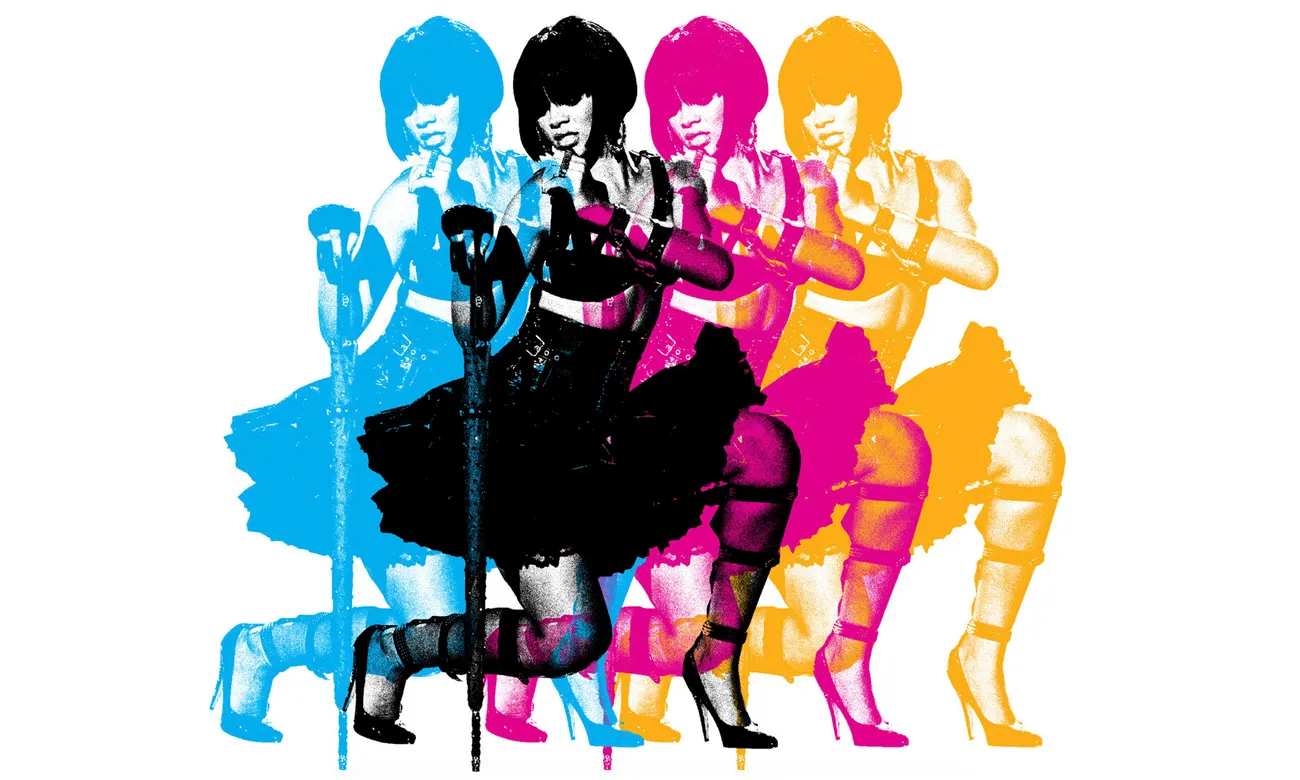
\includegraphics[width=1\textwidth]{misc/title.png}
  \label{titelbild}
\end{figure}

\begin{center}
\textbf{}


\end{center} 

\vspace{1.0cm}


\end{titlepage}
%\restoregeometry

{
\setcounter{tocdepth}{1}
\tableofcontents
}
A collection of hand picked songs. This book is hosted as an online version on \url{https://ratnanil.github.io/Songs/} and includes pdf / epub versions (click on the download symbol). Edits and feedback can be made via the \href{https://github.com/ratnanil/songs}{github repo}. The current version was rendered on 2020-07-12 23:21:47.

\hypertarget{selected-songs}{%
\chapter{Selected Songs}\label{selected-songs}}

\hypertarget{dance-me-to-the-end-of-love---leonard-cohan}{%
\section{Dance me to the end of Love - Leonard Cohan}\label{dance-me-to-the-end-of-love---leonard-cohan}}

\begin{verbatim}

[Am]                          [Em]
Dance me to your beauty with a burning violin
[Am]                               [Em]
Dance me through the panic 'til I'm gathered safely in
[Am]                            [Em]
Lift me like an olive branch and be my homeward dove
[B7]                [Em]
Dance me to the end of love
[B7]                [Em]
Dance me to the end of love

Oh let me see your beauty when the witnesses are gone 
Let me feel you moving like they do in Babylon 
Show me slowly what I only know the limits of 
Dance me to the end of love 
Dance me to the end of love 

Dance me to the wedding now, dance me on and on 
Dance me very tenderly and dance me very long 
We're both of us beneath our love, we're both of us above 
Dance me to the end of love 
Dance me to the end of love

Dance me to your beauty with a burning violin 
Dance me through the panic till I'm gathered safely in 
Touch me with your naked hand or touch me with your glove 
Dance me to the end of love (3x)

{comment: play intro again}
\end{verbatim}

\hypertarget{viva-la-vida---coldplay}{%
\section{Viva la Vida - Coldplay}\label{viva-la-vida---coldplay}}

\begin{verbatim}
{capo: 1}

{start_of_grid}
C - D - G - Em 
{end_of_grid}

(Em)     [C]      [D]
I used to rule the world
          [G]                  [Em]
Seas would rise when I gave the word
                    [C]     [D]
Now in the morning I sleep alone    
         [G]               [Em]
Sweep the streets I used to own

{start_of_grid}
C - D - G - Em    x2
{end_of_grid}

I used to roll the dice 
Feel the fear in my enemy's eyes 
Listen as the crowd would sing 
"Now the old king is dead! Long live the king!" 

One minute I held the key 
Next the walls were closed on me 
And I discovered that my castles stand 
Upon pillars of salt and pillars of sand 

{start_of_chorus}
 [C]            [D]
I hear Jerusalem bells are ringing
[G]          [Em]
Roman Cavalry choirs are singing
[C]             [D]
Be my mirror, my sword, and shield
  [G]               [Em]
My missionaries in a foreign field
[C]              [D]
For some reason I can't explain
[G]                  [Em]            [C]    [D]
Once you go there was never, never an honest word
        [Bm]             [Em]
That was when I ruled the world

{end_of_chours}

It was the wicked and wild wind 
Blew down the doors to let me in 
Shattered windows and the sound of drums 
People couldn't believe what I'd become 

Revolutionaries wait 
For my head on a silver plate 
Just a puppet on a lonely string 
Oh who would ever want to be king? 

{chorus}



\end{verbatim}

\hypertarget{hallelujah---leonard-cohen}{%
\section{Hallelujah - Leonard Cohen}\label{hallelujah---leonard-cohen}}

\begin{verbatim}

Well I heard there was a secret chord 
That David played, and it pleased the Lord 
But you don't really care for music, do ya? 
Well it goes like this 
The fourth, the fifth 
The minor fall and the major lift 
The baffled king composing Hallelujah 
Hallelujah (4x)

Well Your faith was strong but you needed proof 
You saw her bathing on the roof 
Her beauty and the moonlight overthrew you 
she tied you to her kitchen chair 
And she broke your throne and she cut your hair 
And from your lips she drew the Hallelujah 
Hallelujah (4x)

Well baby I've been here before
I've seen this room and I've walked this floor
I used to live alone before I knew ya 
I've seen your flag on the marble arch
Love is not a victory march 
It's a cold and it's a broken Hallelujah 
Hallelujah (4x)

Well there was a time when you let me know
What's really going on below
But now you never show that to me do you?
And remember when I moved in you?
And the holy dove was moving too
And every breath we drew was Hallelujah
Hallelujah (4x)

Well maybe there's a God above
But all I've ever learned from love
Was how to shoot somebody who'd OUT DREW YA
And it's not a cry that you hear at night
It's not somebody who's seen in the light
It's a cold and it's a broken Hallelujah
Hallelujah (repeat... hold...)
\end{verbatim}

\hypertarget{mad-world---gary-jules}{%
\section{Mad World - Gary Jules}\label{mad-world---gary-jules}}

\begin{verbatim}
{year: 2001}

All around me are familiar faces
Worn out places, worn out faces
Bright and early for their daily races
Going nowhere, going nowhere
Their tears are filling up their glasses
No expression, no expression
Hide my head, I want to drown my sorrow
No tomorrow, no tomorrow

And I find it kinda funny, I find it kinda sad
The dreams in which I'm dying are the best I've ever had
I find it hard to tell you, I find it hard to take
When people run in circles it's a very very
Mad world, mad world

Children waiting for the day, they feel good
Happy birthday, happy birthday
Made to feel the way that every child should
Sit and listen, sit and listen

Went to school and I was very nervous
No one knew me, no one knew me
Hello teacher, tell me what's my lesson
Look right through me, look right through me

And I find it kinda funny, I find it kinda sad
The dreams in which I'm dying are the best I've ever had
I find it hard to tell you, I find it hard to take
When people run in circles it's a very very
Mad world, mad world
Enlarge your world
Mad world
\end{verbatim}

\hypertarget{new-slang---the-shins}{%
\section{New Slang - The Shins}\label{new-slang---the-shins}}

\begin{verbatim}

{start_of_grid}
Am C F C G C Am G x4
 C 
{end_of_grid}

[Am]            [C]            [F]
Gold teeth and a curse for this town
[C]           [G]
Were all in my mouth
    [C]          [F]          [Am] [G]
Only I don't know how they got out, dear
[Am]          [C]    [F]
Turn me back into the pet
[C]          [G]
I was when we met
[C]          [F]          [Am] [G]
I was happier then with no mind set

{start_of_chorus}
[G]                   [C]
And if you'd a took to me like
 [F]  [C]          [G]
A gull takes to the wind
           [G]         [C]
Well, I'd a jumped from my tree
   [F]   [C]             [F]         [C]
And I'd a danced like the king of the eyesores
[F]                [C]           [G]
And the rest of our lives would'a fared well
{end_of_chorus}

[Am]              [C]        [F]
New slang when you notice the stripes
[C]             [G]
The dirt in your fries
    [C]                 [F]
Hope it's right when you die
       [Am][G]
Old and bo..ny
[Am]              [C]              [F]
Dawn breaks like a bull through the hall
[C]           [G]
Never should'a called
   [C]             [F]
But my heads to the wall
       [Am][G]
And I'm lonely

{chorus}

[Am]             [C]        [F]
God speed all the baker's at dawn
            [C]       [G]
May they all cut their thumbs
   [C]              [F]
And bleed into their buns
          [Am] [G]
'Till they melt away

{start_of_chorus: Chorus 2}
[G]                   [C]
I'm looking in on the good life
          [F]    [C]      [G]
I might be doomed never to find
                          [C]
Without a trust or flaming fields
    [F] [C]     [G]
[Am] too dumb to refine?
                      [C]
And if you'd a took to me like
    [F]   [C]             [F]          [C]
Well I'd a danced like the queen of the eyesores
[F]                [C]           [G]
And the rest of our lives would'a fared well
{end_of_chorus}
\end{verbatim}

\hypertarget{all-the-world-is-green---tom-waits}{%
\section{All the World is Green - Tom Waits}\label{all-the-world-is-green---tom-waits}}

\begin{verbatim}

[Bm]           [Em]  [A7]            [D]
I fell into the ocean  and you became my wife
[G7]                                        [Bm]
 I risked it all against the sea to have a better life
          [Em]             [A7]         [D]
Marie you are the wild blue sky, men do foolish things
[G7]                                      [Bm]
 You turn kings into beggars and beggars into kings

{start_of_chorus}

  [G]                  [D] 
Pretend that you owe me nothing      
   [A7]             [D]
and all the world is green
[G]                   [D]        
 We can bring back the old days again     
    [A7]             [D]
when all the world is green

{end_of_chorus}

The face forgives the mirror
The worm forgives the plow
The questions begs the answer
Can you forgive me somehow?

Maybe when our story's over
We'll go where it's always spring
The band is playing our song again
And all the world is green [Play Chorus]

The moon is yellow silver
On the things that summer brings
It's a love you'd kill for
And all the world is green

He's balancing a diamond
On a blade of grass
The dew will settle on our graves
When all the world is green

{Comment: Play chorus, solo, repeat last verse}
\end{verbatim}

\hypertarget{wagon-wheel---old-crow-medicine-show}{%
\section{Wagon Wheel - Old Crow Medicine Show}\label{wagon-wheel---old-crow-medicine-show}}

\begin{verbatim}
{capo: 2}

[G]                     [D]
Headed down south to the land of the pines
       [Em]                 [C]
And I'm thumbin' my way into North Caroline
[G]
Starin' up the road
           [D]       [C]
And pray to God I see headlights


I made it down the coast in seventeen hours 
Pickin' me a bouquet of dogwood flowers 
And I'm a hopin' for Raleigh 
I can see my baby tonight

{start_of_chorus}
  [G]                 [D]
So rock me mama like a wagon wheel
[Em]           [C]
Rock me mama anyway you feel
[G][D]   [C]
Hey, mama rock me
[G]                  [D]
Rock me mama like the wind and the rain
[Em]               [C]
Rock me mama like a south-bound train
[G][D]   [C]
Hey, mama rock me
{end_of_chorus}

Intro

Runnin' from the cold up in New England
I was born to be a fiddler in an old-time stringband
My baby plays the guitar
I pick a banjo now

Oh, the North country winters keep a gettin' me now
Lost my money playin' poker so I had to up and leave
But I ain't a turnin' back
To livin' that old life no more

{chorus}

Walkin' to the south out of Roanoke
I caught a trucker out of Philly
Had a nice long toke
But he's a headed west from the Cumberland Gap
To Johnson City, Tennessee

And I gotta get a move on before the sun
I hear my baby callin' my name
And I know that she's the only one
And if I die in Raleigh
At least I will die free

{chorus}
\end{verbatim}

\hypertarget{for-the-windows-in-paradise---sufjan-stevens}{%
\section{For the Windows in Paradise - Sufjan Stevens}\label{for-the-windows-in-paradise---sufjan-stevens}}

\begin{verbatim}
{year: 2003}

[Am]         Fmaj7    [C]             [G]
I have called you children, I have called you son,
[Am]        Fmaj7     [C]         [G]
What is there to answer when I'm the only one?
[Am]        Fmaj7   [C]           [G]
Morning comes in paradise, morning comes in light,
[Am]    Fmaj7   [C] [G]
Still I must obey, still I must invite.

          [Am]       Fmaj7       [C]  [G]
If there's anything to say, if there's anything to do,
          [Am]     Fmaj7  [C]      [G]
If there's any other way, I'll do anything for you.

I was dressed embarrassment. 
I was dressed in wine. 
If you had a part of me, will you take you're time? 
Even if I come back, even if I die 
Is there some idea to replace my life? 

Like a father to impress; 
Like a mother's mourning dress, 
If you ever make a mess, I'll do anything for you 

I have called you preacher; I have called you son. 
If you have a father or if you haven't one, 
I'll do anything for you (4x)

I did everything for you (repeat.. about 8x)
\end{verbatim}

\hypertarget{build-me-up-buttercup---the-foundations}{%
\section{Build me up Buttercup - The Foundations}\label{build-me-up-buttercup---the-foundations}}

\begin{verbatim}


{start_of_chorus}
Why do you build me up (build me up) Buttercup, baby
Just to let me down (let me down)and mess me around
And then worst of all (worst of all) you never call, baby
When you say you will (say you will) but I love you still
I need you (I need you) more than anyone, darlin'
You know that I have from the start
So build me up (build me up) Buttercup, 
don't break my heart
{end_of_chorus}

"I'll be over at ten", you told me time and again
But you're late, I wait around and then (bah-dah-dah)
I run to the door, I can't take any more
It's not you, you let me down again

{start_of_bridge}
(Hey, hey, hey!) Baby, baby, try to find
(Hey, hey, hey!)[A]little time, and I'll make you happy
(Hey, hey, hey!) I'll be home
I'll be beside the phone waiting for you
Ooo-oo-ooo, ooo-oo-ooo
{end_of_bridge}

{chorus}

You were my toy but I could be the boy you adore
If you'd just let me know (bah-dah-dah)
Although you're untrue, I'm attracted to you all the more
Why do I need you so

{bridge}

{chorus}

\end{verbatim}

\hypertarget{i-will-follow-you-into-the-dark---death-cab-for-cutie}{%
\section{I will follow you into the Dark - Death Cab for Cutie}\label{i-will-follow-you-into-the-dark---death-cab-for-cutie}}

\begin{verbatim}
{capo: 5}

[C]
Love of mine
                [Am](D root note)
Someday you will die
                     [F]
But I will be close behind
          [C]                [G]
I will follow, you into the dark

No blinding light
Or tunnels to gates of white
Just our hands clasped so tight
Waiting for, the hint of a spark 

{start_of_chorus} 
  [Am]               [C]     
If heaven and hell decide,      
          [F]         [C]G
that they both are satisfied
[Am]            [C]                G(bar)
Illuminate the "no's", on their vacancy signs
[Am]                     [C]
If there's no one beside you,
          [E]    [Am]G
when your soul embarks
Bb                 Bbm           [F](C root note)
Then I will follow you into the dark
{end_of_chorus}

Catholic school
As vicious as roman rule
I got my knuckles bruised 
By a lady in black
     
And I held my tongue 
as she told me "son, fear is the heart of love." 
So I never went back

{chorus}

You and me, have seen everything to see
From Bangkok to Calgary  
And the soles of your shoes
 
Are all worn down, the time for sleep is now
But it's nothing to cry about  
Because we'll hold each other soon
[Am]                 Fm    Fm
in the blackest of rooms 

[Am]                [C]    
If heaven and hell decide, 
          [F]          [C]G
that they both are satisfied
[Am]            [C]                G(bar)
Illuminate the "no's", on their vacancy signs
[Am]                     [C]            [E]    [Am]G
If there's no one beside you, when your soul embarks
[F]               Fm           [C]   
Then I will follow you into the dark

{start_of_tab}
E---------------------|
B---1---1--------1----|
G---2---2--------2----|
D---0---0--------2----|
A---3---2----0---0----|
E---------------------|
{end_of_tab}

[F]               Fm           [C]   
Then I will follow you into the dark

\end{verbatim}

\hypertarget{guitar-classics}{%
\chapter{Guitar Classics}\label{guitar-classics}}

\hypertarget{winds-of-change---scorpions}{%
\section{Winds of Change - Scorpions}\label{winds-of-change---scorpions}}

\begin{verbatim}
{year: 1991}

{start_of_grid}
 F  Dm  F   Dm Am   G  Am  G  C   C
{end_of_grid}

[C]            [Dm]
I follow the Moskva
             [C]
Down to Gorky Park
                [Dm]     [Am] [G][C] 
Listening to the wind of change

[C]             [Dm]
An August summer night
                [C]
Soldiers passing by
                [Dm]     [Am] [G][C] 
Listening to the wind of change

The world is closing in
Did you ever think
That we could be so close, like brothers

The future's in the air
I can feel it everywhere
Blowing with the wind of change 

[C] [G]       [Dm]         [G]
Take me to the magic of the moment
    [C]   [G]
On a glory night
         [Dm]          [G]           [Am]
Where the children of tomorrow dream away
[F]             [G]
In the wind of change
Walking down the street
Distant memories
Are buried in the past forever


I follow the Moskva
Down to Gorky Park
Listening to the wind of change
Chorus (1st Part):
Take me to the magic of the moment
On a glory night
Where the children of tomorrow share their dreams
With you and me

Take me to the magic of the moment
On a glory night
Where the children of tomorrow dream away
In the wind of change

{start_of_bridge}
[Am]                     [G]
The wind of change blows straight
                 [Am]
Into the face of time
                          [G]
Like a stormwind that will ring
                             [Am]
The freedom bell for peace of mind
                  [C]
Let your balalaika sing
                       [Em]    [E7]
What my guitar wants to say
{end_of_bridge}

{chorus}
{comment: play outro, same as intro}
\end{verbatim}

\hypertarget{sweet-home-alabama---lynyrd-skynyrd}{%
\section{Sweet Home Alabama - Lynyrd Skynyrd}\label{sweet-home-alabama---lynyrd-skynyrd}}

\begin{verbatim}

{start_of_tab}
e|-------------------------3-|
B|-----3---------3---------3-|
G|-------2----------0------0-|  x4
D|-0-0---------------------0-|     
A|----------3-3------------2-|
E|---------------------3-3-3-|
{end_of_tab}

[D] [Cadd9]       [G]
Big wheels keep on turning
[D]     [Cadd9]        [G]
Carry me home to see my kin
[D]    [Cadd9]         [G]
Singing songs about the south land
[D]     [Cadd9]        [G]                           
I miss 'ole' 'bamy once again and I think it's a sin

[D]             [Cadd9]          [G]
Well I heard Mr. Young sing about her
[D]             [Cadd9]      [G]
Well I heard old Neil put her down
[D]             [Cadd9]    [G]
Well I hope Neil Young will remember
[D]       [Cadd9]            [G]               
[A]outhern man don’t need him around, anyhow

[Chorus]

{start_of_chorus}
[D]  [Cadd9] [G]   [D]       [Cadd9]      [G]        
Sweet home Alabama, where the skies are so blue
[D]  [Cadd9] [G]   [D]       [Cadd9]       [G]     
Sweet home Alabama, lord I’m coming home to you.
{end_of_chorus}

[F]
[D]add9[G]
[D]add9[G]

[D]      [Cadd9]           [G]      [F] [C] [D]
In Birmingham they love the Gov'nor, boo-hoo-hoo
[D]       [Cadd9]           [G]
Now we all did what we could do
[D]      [Cadd9]     [G]
Now watergate doesn't bother me
[D]      [Cadd9]          [G]
Does you conscience bother you, (now tell the truth!)

{chorus}

[D][Cadd9]                   [G]
Now Muscle Shoals has got the Swappers
[D]             [Cadd9]                 [G]
And they've been known to pick a song or two (yes we do)
[D]      [Cadd9]       [G]
Lord they get me off so much
[D]         [Cadd9]            [G]   
They pick me up when I'm feeling blue, Now how about you?

{chorus}

[D]  [Cadd9] [G]     
Sweet home Alabama (Oh sweet home baby)
[D]      [Cadd9]      [G]   
Where the skies are so blue (And the governor's true)
[D]  [Cadd9] [G]
Sweet Home Alabama, (Lord, yeah)
[D]      [Cadd9]        [G]
Lord, I'm coming home to you
\end{verbatim}

\hypertarget{calafornia-dreaming---the-mamas-and-the-papas}{%
\section{Calafornia Dreaming - the Mamas and the Papas}\label{calafornia-dreaming---the-mamas-and-the-papas}}

\begin{verbatim}


    NC/(Em)          [Am]      [G]        [F]
All the leaves are brown (all the leaves are brown)
       [G]    [Am]                   [E]
And the sky is gray  (and the sky is gray)
      [F]             [C]        [E]  [Am]
I've been for a walk  (I've been for a walk)
     [F]      [Am]                [E]
On a winter's day  (on a winter's day)
       [E]             [Am]    [G]      [F]
I'd be safe and warm (I'd be safe and warm)
    [G]    [Am]               [E]
If I was in L.A.  (if I was in L.A.)

{start_of_chorus}
[E]          [Am]     [G]       [F]
California dreamin  (California dreamin')
   [G]    [Am]     [E]
On such a winter's day
{end_of_chorus}


[E]            [Am]
Stopped in to a church
 [G]          [F]
I passed along the way
       [G]            [Am]            [E]
Well I got down on my knees (got down on my knees)
[F]             [Am]               [E]
And I pretend to pray (I pretend to pray)
[E]                  [Am]      [G]                [F]
You know the preacher likes the cold (preacher likes the cold)
        [G]       [Am]                  [E]
He knows I'm gonna stay (knows I'm gonna stay)

{chorus}

[E]              [Am]      [G]        [F]
All the leaves are brown (all the leaves are brown)
       [G]    [Am]                   [E]
And the sky is gray (and the sky is gray)
[F]            [C]        [E]  [Am]
I've been for a walk (I've been for a walk)
    [F]      [Am]                [E]
On a winter's day  (on a winter's day)
       [E]             [Am]    [G]      [F]
If I didn't tell her  (if I didn't tell her)
       [G]   [Am]                 [E]
I could leave today (I could leave today)

[E]          [Am]     [G]       [F]
California dreamin (California dreamin')
  [G]    [Am]     [E]          [G]      [F]
On such a winter's day (California dreamin')
  [G]    [Am]     [E]          [G]      [F]
On such a winter's day (California dreamin')
  [G]    [Am]     [E]   [Am]
On such a winter's day
\end{verbatim}

\hypertarget{ein-bett-im-kornfeld---jurgen-drews}{%
\section{Ein Bett im Kornfeld - Jürgen Drews}\label{ein-bett-im-kornfeld---jurgen-drews}}

\begin{verbatim}

[D]
Sommerabend über blühendem Land.
Schon seit Mittag stand ich am 
Straßenrand.
           [A]
Bei jedem Wagen, der vorüber fuhr,
            [D]
hob ich den Daumen.
auf einem Fahrrad kam da ein 
Mädchen her.
Und sie sagte: "Ich bedaure dich sehr."
          [A]                                         [D]
Doch ich lachte und sprach: "Ich brauch keine weichen Daunen"

{start_of_chorus}
             [G]
Ein Bett im Kornfeld,
Das ist immer frei, denn es ist
[D]
Sommer, und was ist schon dabei.
            [A]
Die Grillen singen und es duftet 
                   [D]
nach Heu, wenn ich träume.
             [G]
Ein Bett im Kornfeld, zwischen 
Blumen und Stroh,
         [D]
Und die Sterne leuchten mir sowieso
             [A]
Ein Bett im Kornfeld mach ich mir 
               [D]
irgendwo ganz alleine.

{end_of_chorus}

[D]
Etwas später lag ihr Fahrrad im 
Gras, Und so kam es, dass sie die 
Zeit vergass,
         [A]
Mit der Gitarre hab ich ihr erzählt
           [D]
Von meinem Leben.
Auf einmal rief sie
"Es ist höchste Zeit, Schon ist es 
dunkel und mein Weg ist noch Weit"
          [A]
Doch ich lachte und sprach:
                           [D]
"Ich hab dir noch viel zu geben".

{chorus}

\end{verbatim}

\hypertarget{boulevard-of-broken-dreams---green-day}{%
\section{Boulevard of Broken Dreams - Green Day}\label{boulevard-of-broken-dreams---green-day}}

\begin{verbatim}

[Em]     [G]            [D]            [A]           [Em]
I walk a lonely road, the only one that I have ever known
           [G]           [D]              [A]             [Em]
Don't know where it goes, but it's home to me and I walk alone

{start_of_grid}
Em__|G___|D___|A___| 
{end_of_grid}

I walk this empty street, on the boulevard of broken dreams
Where the city sleeps, and I'm the only one and I walk alone


[Em][G][D]          [A]         [Em]
.........I walk alone, I walk alone.
[Em][G][D]          [A]
.........I walk alone, I walk a....


{start_of_chorus}
[C]    [G]          [D]            [Em]
    My shadow's the only one that walks beside me
[C]     [G]     [D]             [Em]
    My shallow heart's the only thing that's beating
[C]     [G]     [D]               [Em]
    Sometimes I wish someone out there will find me
[C]      [G]    [B7]
    Till then I walk alone
{end_of_chorus}


[Em]  [G]   [D]     [A]
Ah-Ah Ah-Ah Ah-Ah   Ahhh-Ah
    [Em] [G]   [D]     [A]
haaa-ah  Ah-Ah Ah-Ah   Ah-Ah


I'm walking down the line
That divides me somewhere in my mind
On the border line of the edge
And where I walk alone

{start_of_grid}
Em G  D  A
{end_of_grid}

Read between the lines
What's fucked up and everything's all right
Check my vital signs, to know I'm still alive
And I walk alone


I walk alone, I walk alone.
I walk alone, I walk a....


{chorus}


Ah-Ah Ah-Ah Ah-Ah   Ahhh-Ah
haaa-ah  Ah-Ah Ah-Ah  I walk alone, I walk a...


{start_of_grid}
 C G  D  Em 
 C G  D  Em 
 C G  D  Em 
 C G  B  B7 
{end_of_grid}


I walk this empty street, on the boulevard of broken dreams
Where the city sleeps, and I'm the only one and I walk a...


{chorus}

\end{verbatim}

\hypertarget{lemon-tree---fools-garden}{%
\section{Lemon Tree - Fools Garden}\label{lemon-tree---fools-garden}}

\begin{verbatim}
{year: 1996}

{start_of_grid}
Em__|Bm__|Em__|Bm__|
Am__|Bm__|Em__|Bm_E|
{end_of_grid}

[Em]             [Bm]
I'm Sitting Here In[A]Boring Room
[Em]                          [Bm]
It's Just Another Rainy Sunday Afternoon
[Em]                     [Bm]
I'm Wasting My Time I Got Nothing To Do
[Em]                  [Bm]
I'm Hanging Around I'm Waiting For You
   [Am]                 [Bm]    [Em] [Bm][Em]
But Nothing Ever Happens - And I Wonder

I'm Driving Around In My Car
I'm Driving Too Fast I'm Driving Too Far
I'd Like To Change My Point Of View
I Feel So Lonely I'm Waiting For You
But Nothing Ever Happens - And I Wonder

Chorus
[G]           [D]
I Wonder How I Wonder Why
[Em]                           [Bm]
Yesterday You Told Me 'bout The Blue Blue Sky
[C]               [D]                  [G]       [D]
And All That I Can See Is Just[A]Yellow Lemon-tree
[G]                [D]
I'm Turning My Head Up And Down
[Em]                                [Bm]
 I'm Turning Turning Turning Turning Turning Around
[C]               [A]                  [D]
And All That I Can See Is Just another Lemon-tree


{start_of_bridge}
 Em Bm Em Bm Am Bm Em 
 dadada....
{end_of_bridge}


I'm Sitting Here I Miss The Power
I'd Like To Go Out Taking a Shower
But There's a Heavy Cloud Inside My Head
I Feel So Tired Put Myself Into Bed
Where Nothing Ever Happens - And I Wonder

[B]         [Em]
Isolation - Is Not Good For Me
[D]        [G]              [B]
Isolation - I Don't Want To Sit On a Lemon-tree

I'm Steppin' Around In a Desert Of Joy
Baby Anyhow I'll Get Another Toy
And Everything Will Happen - And You'll Wonder

Chorus 2x

[C]               [D]
And All That I Can See
[C]               [D]
And All That I Can See
[C]               [D]
And All That I Can See
                [G]
Is Just a Yellow Lemon-tree.

\end{verbatim}

\hypertarget{sound-of-silence---simon-and-garfunkel}{%
\section{Sound of Silence - Simon and Garfunkel}\label{sound-of-silence---simon-and-garfunkel}}

\begin{verbatim}
{year: 1964}
{capo: 6}

[Am]                    [G]
Hello darkness, my old friend,
                          [Am]
I've come to talk with you again,
                 [F]   [C]         
Because a vision softly creeping,
        [Am]           [F]   [C]                 
Left its seeds while I was sleeping,
        [F]                             [C]   
And the vision that was planted in my brain
      [Am]      
Still remains
            [G]     [Am]              
Within the sound of silence.

[Am]                        [G]        
In restless dreams I walked alone
                       [Am]
Narrow streets of cobblestone,
[Am]               [F]      [C]
'Neath the halo of a street lamp,
             [Am]         [F]      [C]
I turned my collar to the cold and damp
       [F]                                       [C]    
When my eyes were stabbed by the flash of a neon light
              [Am]
That split the night
               [G]      [Am]
And touched the sound of silence.

[Am]                      [G]
And in the naked light I saw
                          [Am]
Ten thousand people, maybe more.
[Am]             [F]     [C]
People talking without speaking,
[Am]                 [F]     [C]
People hearing without listening,
                [F]                     [C]
People writing songs that voices never share
          [Am]
And no one dare
            [G]      [Am]
Disturb the sound of silence.

[Am]                      [G]
Fools said I, you do not know
                     [Am]
Silence like a cancer grows.
[Am]                  [F]        [C]
Hear my words that I might teach you,
[Am]                 [F]         [C]
Take my arms that I might reach you.
        [F]                        [C]
But my words like silent raindrops fell,
     [Am]
And echoed
      [G]      [Am]
In the wells of silence

[Am]                     [G]
And the people bowed and prayed
                    [Am]
To the neon God they made.
[Am]                      [F]    [C]
 And the sign flashed out its warning,
[Am]                  [F]   [C]
In the words that it was forming.
        [Am]            [F]
And the sign said, the words of the prophets
       [F]                  [C]
Are written on the subway walls
              [Am]
And tenement halls.
                     [G]       [Am]     
And whispered in the sounds of silence.
\end{verbatim}

\hypertarget{blowing-in-the-wind---bob-dylan}{%
\section{Blowing in the Wind - Bob Dylan}\label{blowing-in-the-wind---bob-dylan}}

\begin{verbatim}

[C]       [F]        [C]      [Am] 
How many roads must a man walk down, 
  [C]        [F]  [G]-[G7]
before you call him a man?
[C]     [F]          [C]       [Am] 
How many seas must a white dove sail, 
  [C]        [F]        [G]-[G7]
before she sleeps in the sand?
[C]     [F]               [C]  [Am]
How many times must the cannonballs fly, 
  [C]           [F]    [G]
before they're forever banned?
      [F]       [G]      C-E-Am             
The answer my friend, is blowing in the wind.
      [F]       [G]         [C]
The answer is blowing in the wind.

How many years must a mountain exist, 
before it is washed to the sea?
How many years can some people exist, 
before they're allowed to be free? 
How many times can a man turn his head, 
and pretend that he just doesn't see?
The answer my friend, is blowing in the wind.
The answer is blowing in the wind.

How many times must a man look up, 
before he can see the sky?
How many ears must one man have, 
before he can hear people cry?
How many deaths will it take 'till he knows, 
that too many people have Died?
The answer my friend, is blowing in the wind.
The answer is blowing in the wind.

\end{verbatim}

\hypertarget{moring-has-broken---cat-stevens}{%
\section{Moring has broken - Cat Stevens}\label{moring-has-broken---cat-stevens}}

\begin{verbatim}

           [C]   Dm [G]            [F]  [C]
Morning has brok-en, like the first morn-ing
[C]          [Em] [Am][D7]           [G] [G]
Blackbird has spok-en, like the first bird
[C]           [F]  [F]  [C]            [Am] [D]
Praise for the sing-ing, praise for the morn-ing
[G]            [C]    [F] [G]            [C]
Praise for them spring-ing fresh from the world

                [C]  Dm   [G]         [F]  [C]
Sweet the rain's new fall, sunlit from heav-en
[C]           [Em][Am]  [D7]         [G]  [G]
Like the first dew fall, on the first grass
[C]           [F]   [F]  [C]        [Am] [D]
Praise for the sweet-ness of the wet gard-en
[G]      [C]      [F]  [G]            [C]
Sprung in complete-ness where his feet pass

           [D] [Em]  [A]         [G]  [D]
Mine is the sunlight, mine is the morn-ing
[D]        [F#m]Bm    [E]      [A] [A]
Born of the one light, Eden saw play
[D]        [G] [G]   [D]          [Bm] [E]
Praise with ela-tion, praise every morn-ing
[A]  [D]    [G]  [A]        [D]
God's recrea-tion of the new day

           [C]   Dm [G]            [F]  [C]
Morning has brok-en, like the first morn-ing
[C]          [Em] [Am][D7]           [G] [G]
Blackbird has spok-en, like the first bird
[C]           [F]  [F]  [C]            [Am] [D]
Praise for the sing-ing, praise for the morn-ing
[G]            [C]    [F] [G]            [C]
Praise for them spring-ing fresh from the world
\end{verbatim}

\hypertarget{dust-in-the-wind---kansas}{%
\section{Dust in the Wind - Kansas}\label{dust-in-the-wind---kansas}}

\begin{verbatim}

{start_of_tab}
e|-----------|
B|-1-------1-|
G|-----0-----|
D|---2-------|
A|-3-----3---|
E|-----------|
{end_of_tab}


 [C]    G/B [Am]  [G]        Dm           [Am]
I close my eyes only for a moment and a moment´s gone.
[C] G/B  [Am]   [G]            Dm         [Am]
All my dreams pass before my eyes a curiosity.

{start_of_chorus}
[D][G]      [Am]  [D]          [G]         [Am]
Dust in the wind, all we are is dust in the wind.
{end_of_chorus}


[C]G/B [Am]  [G]            Dm             [Am]
Same old song, just a drop of water in the endless sea.
[C] G/B [Am] [G]                Dm               [Am]
All we do, crumbles to the ground though we refuse to see.

{chorus}

[C]    G/B  [Am] [G]               Dm            [Am]
Don't hang on, nothing last´s forever but the earth and sky.
[C]G5     [Am][G]                 Dm        [Am]
It slips away all your money won´t another minute buy.

{chorus}
{chorus}

\end{verbatim}

\hypertarget{house-of-the-rising-sun---the-animals}{%
\section{House of the Rising Sun - The Animals}\label{house-of-the-rising-sun---the-animals}}

\begin{verbatim}
{year: 1964}

{start_of_grid}
INTRO-  Am, C, D, F, Am, E, Am , E 
{end_of_grid}

     [Am] [C]      [D]         [F]
There is a house in New Orleans
    [Am]     [C]    [E]  [E7]
They call the Risin' Sun
        [Am]     [C]     [D]         [F]
And it's been the ruin of many a poor boy.
   [Am]   [E]      [Am]
And God, I know I'm one.

My mother was a tailor.
She sewed my new blue jeans.
My father was a gamblin' man
Down in New Orleans.

{start_of_grid}
 C, D, F, Am, E, Am , E 
{end_of_grid}

Now, the only thing a gambler needs
Is a suitcase and a trunk
And the only time that he's satisfied
Is when he's on a drunk

Oh, Mothers, tell your children
Not to do what I have done.
Spend your lives in sin and misery
In the house of the risin' sun.

Well, I've got one foot on the platform.
the other foot on the train.
I'm goin' down to New Orleans
To wear that ball and chain.

{comment: Play first verse again}

\end{verbatim}

\hypertarget{hurt---johnny-cash}{%
\section{Hurt - Johnny Cash}\label{hurt---johnny-cash}}

\begin{verbatim}

[Am][C]     [D]   [Am]     [C]    [D]     [Am]
   I hurt myself today   to see if I still feel
 [C]  [D]      [Am]      [C]    [D]        [Am]
I focus on the pain   the only thing that's real
   [C]    [D]     [Am]       [C]    [D]     [Am]
The needle tears a hole   the old familiar sting
      [C]    [D]    [Am]         [C]    [D]    [G]         
Try to kill it all away   but I remember everything

{start_of_chorus}
[Am]           [F]   [C]             [G]
What have I become?     My sweetest friend
[Am]       [F]           [C]      [G]
Everyone I know  goes away in the end
   [Am]               [F]  [G]             [G]
And you could have it all   My empire of dirt
[Am]           [F]    [G]              [Am]
I will let you down    I will make you hurt
{end_of_chorus}

I wear this crown of thorns   upon my liar's chair
Full of broken thoughts   I cannot repair
Beneath the stains of time   the feelings disappear
You are someone else   I am still right here

{chorus}

  [Am]             [F]   [G]            [G]
If I could start again  a million miles away
[Am]           [F]  [G]
I would keep myself  I would find a way
\end{verbatim}

\hypertarget{streets-of-london---ralph-mctell}{%
\section{Streets of London - Ralph McTell}\label{streets-of-london---ralph-mctell}}

\begin{verbatim}
{year: 1967}

[C]              [G]      [Am]               [Em]
Have you seen the old man, in the closed-down market
[F]           [C]              [D7]     [G7]
picking up the papers, with his worn-out shoes?
[C]            [G]           [Am]             [Em]
In his eyes you see no pride, and held loosely by his side
[F]        [C]             [G7]        [C]
yesterday's papers, telling yesterday's news

{start_of_chorus}
     [F]         [Em]            [C]  [G7]   [Am]
    So how can you tell me, you're lo - ne - ly
[D7]         [D7]                   [G]    [G7]
  and say for you that the sun don't shine?
[C]            [G]              [Am]                 [Em]
Let me take you by the hand, and lead you through the streets of London
[F]            [C]           [G7]                 [C]    [C]
  I'll show you something, to make you change your mind
{end_of_chorus}

Have you seen the old gal, who walks the streets of London
dirt in her hair, and her clothes in rags?
She's no time for talking, she just keeps right on walking
Carrying her home, in two carrier bags

{chorus}

And in the all-night cafe, at a quarter past eleven
some old man sitting there, all on his own
Looking at the world, over the rim of his tea-cup
Each day lasts an hour, then he wanders home alone

{chorus}

And have you seen the old man, outside the seaman's mission?
His memory's fading, with those medal ribbons that he wears
And in our winter city, the rain cries little pity
For one more forgotten hero, and a world that doesn't care

\end{verbatim}

\hypertarget{mundart-und-deutsch}{%
\chapter{Mundart und Deutsch}\label{mundart-und-deutsch}}

\hypertarget{heidi---mani-matter}{%
\section{Heidi - Mani Matter}\label{heidi---mani-matter}}

\begin{verbatim}

{time: 4/8}
{start_of_grid}
|Am______|Dm__Am__|____F___|____Am__|
|________|Dm__Am__|E___Am__|____E7__|
|C_______|G7______|C_______|G7__C___|
{end_of_grid}

Är wohnt a dr glyche Gass
Und i bi mit dir i d'Klass
So ischs cho, das mir grad beidi
Ds Härz a di verlore hei
Heidi, mir wei di beidi
Beidi, Heidi, hei di gärn

Är isch grosse Held im Sport
I probieres meh mit Wort
Jeden uf sy Art umwärbe
Mir di, Heidi, ig und är
Heidi, mir wei di beidi
Beidi, Heidi, hei di gärn

Zum Bewys är heig di gärn
Schiesst är Gool bi FC Bärn
Ig erkläre mi dir schlicht
I Form vo lyrische Gedicht
Heidi, mir wei di beidi
Beidi, Heidi, hei di gärn

Jede Sunntig dänksch am Mätsch
Är syg dä wo d'lieber hätsch
Findsch daheim vo mir e Brief
De chehrt sech ds Blatt, du süfzgisch tief
Heidi, mir wei di beidi
Beidi, Heidi, hei di gärn

S'het nid chönne wytergah
Hesch nid beidi chönne ha
Schliesslech hei du är und i gseit
Heidi, jitz entschliessisch di
Heidi, entscheid di, beidi
Wei di, beidi chasch nid ha

Hätti gwüsst wis usechunnt
Einisch ire schwache Stund
Hesch du di verlobt, s'isch zvil
Mit ihm am Sunntig nach em Spil
Nei, di Entscheidig, Heidi
Nei dy Bscheid - i bi enttüüscht

{start_of_grid}
|Am______|Dm__Am__|____F___|____Am__|
|________|Dm__Am__|E___Am__|E___Am__|
{end_of_grid}


Dadrus han i glehrt, dass hütt
Nümm so vil erreicht, wär d'Lüt
Mit Literatur erchlüpft
Wi wär a ds rächten Ort hi stüpft
\end{verbatim}

\hypertarget{arabisch---mani-matter}{%
\section{Arabisch - Mani Matter}\label{arabisch---mani-matter}}

\begin{verbatim}
{time: 2/4}

{start_of_grid}
|Am______|________|________|________|
|Am______|________|________|________|
|Dm______|________|Am______|________|
|E_______|________|Am______|________|
{end_of_grid}

Dr Sidi Abdel Assar vo El Hama
Het mal am Morge früe no im Pijama
Ir Strass vor dr Moschee
Zwöi schöni Ouge gseh
Das isch dr Afang worde vo sim Drama

S isch d Tochter gsy vom Mohamed Mustafa
Dr Abdel Assar het nümm chönne schlafa
Bis är bim Mohamed
Um d Hand aghalte hed
Und gseit: I biete hundertfüfzig Schaf a

Dr Mohamed het gantwortet: Bi Allah
Es fröit mi, dass my Tochter dir het gfalla
Doch wärt isch si, my Seel
Zwöhundertzwänzg Kamel
Und drunder chan i dir sen uf ke Fall la

Da het dr Abdel Assar gseit: O Sidi
Uf sone tüüre Handel gang i nid y
Isch furt, het gly druf scho
[E]illigeri gno
Wo nid so schön isch gsy, drfür e gschydi

Doch wenn es Nacht wird über der Sahara
Luegt är dr Mond am Himel häll und klar a
Und truuret hie und da
De schönen Ouge na
Und dänkt: Hätt i doch früecher afa spara
\end{verbatim}

\hypertarget{hemmige---mani-matter}{%
\section{Hemmige - Mani Matter}\label{hemmige---mani-matter}}

\begin{verbatim}
{capo: 1}
{time: 4/4}
{start_of_grid}
|Em______|Am______|D7______|G_______|
|________|H7______|Em______|H7______|
{end_of_grid}


S'git Lüt, die würden alletwäge nie
Es Lied vorsinge, so win ig jitz hie
Eis singen um kei Prys, nei bhüetis nei
Wil si Hemmige hei

Si wäre vilicht gärn im Grund gno fräch
Und dänke, das syg ires grosse Päch
Und s'laschtet uf ne win e schwäre Stei
Dass si Hemmige hei

I weis, das macht eim heiss, verschlat eim d'Stimm
Doch dünkt eim mängisch o s'syg nüt so schlimm
S'isch glych es Glück, o we mirs gar nid wei
Das mir Hemmige hei

Was unterscheidet d'Mönsche vom Schimpans
S'isch nid die glatti Hut, dr fählend Schwanz*
Nid dass mir schlächter d'Böim ufchöme, nei
Dass mir Hemmige hei

Me stell sech d'Manne vor, wenns anders wär
Und s'chäm es hübsches Meiteli derhär
Jitz luege mir doch höchstens chly uf d'Bei
Wil mir Hemmige hei

{start_of_grid: Abschluss}
|Em______|Am______|D7______|G_______|
|________|H7______|Em__H7__|Em______| 
{end_of_grid}

Und we me gseht, was hütt dr Mönschheit droht
So gseht me würklech schwarz, nid nume rot
Und was me no cha hoffen isch alei
Dass si Hemmige hei
\end{verbatim}

\hypertarget{kinder---sind-so-kleine-hande---bettina-wegner}{%
\section{Kinder - Sind so kleine Hände - Bettina Wegner}\label{kinder---sind-so-kleine-hande---bettina-wegner}}

\begin{verbatim}

{start_of_grid}
Am______|Dm______|E________|Am______|
Am______|Dm______|E________|Am______|
C_______|G_______|_________|Am______|
C_______|G_______|_________|Am______|
{end_of_grid}

Sind so kleine Hände, winz’ge Finger dran.
Darf man nie drauf schlagen, die zerbrechen dann.
Sind so kleine Füße, mit so kleinen Zeh’n.
Darf man nie drauf treten, könn’ sie sonst nicht gehn.

Sind so kleine Ohren; scharf, und ihr erlaubt.
Darf man nie nie zerbrüllen, werden davon taub.
Sind so schöne Münder, sprechen alles aus.
Darf man nie verbieten, kommt sonst nichts mehr raus.

Sind so klare Augen, die noch alles sehn.
Darf man nie verbinden, könn’ sie nichts verstehn.
Sind so kleine Seelen, offen und ganz frei.
Darf man niemals quälen, geh’n kaputt dabei.

Ist so’n kleines Rückgrad, sieht man fast noch nicht.
Darf man niemals beugen, weil es sonst zerbricht.
Grade, klare Menschen wär’n ein schönes Ziel.
Leute ohne Rückgrad hab’n wir schon zuviel.
\end{verbatim}

\hypertarget{bim-coiffeur---mani-matter}{%
\section{Bim Coiffeur - Mani Matter}\label{bim-coiffeur---mani-matter}}

\begin{verbatim}

{time: 4/4}

{start_of_grid}
|C_______|____Am__|Dm______|____G7__|
|C_______|____Am__|Dm______|G7______|
{end_of_grid}

Bim Coiffeur bin i gsässe vor em Spiegel, luege dry
Und gseh dert drinn e Spiegel wo ar Wand isch vis-a-vis
Und dert drin spieglet sech dr Spiegel da vor mir
Und i däm Spiegel widerum dr Spiegel hindefür

Und so geng wyter, s'isch gsy win e länge Korridor
I däm my Chopf gwüss hundertfach vo hinden und vo vor
Isch ufgreit gsy i eier Kolonne, z'hinderscht isch dr Chopf
I ha ne nümme gchennt, so chly gsy win e Gufechnopf

My Chopf, dä het sich dert ir Wyti, stellet öich das vor
Verloren ir Unäntlechkeit vom länge Korridor
I ha mi sälber hinde gseh verschwinde, ha das gseh
[Am]eiterhälle Vormittag und wi we nüt wär gscheh

Vor Chlupf han i mys Muul ufgscperrt, da sy im Korridor
Grad hundert Müüler mit ufgange win e Männerchor
[E]ännerchor us mir alei, es cheibe gspässigs Gfüel
Es metaphysischs Grusle het mi packt im Coiffeurgstüel

{start_of_grid}
|C_______|____Am__|Dm______|____G7__|
|C_______|____Am__|Dm__G7__|____C___| 
{end_of_grid}

I ha d'Serviette vo mer grissen, ungschore sofort
Das Coiffeurgschäft verla mit paar entschuldigende Wort
Und wenn dir findet i sött e chly meh zum Coiffeur ga
De chöit dir jitz verstah warum i da e Hemmig ha


\end{verbatim}

\hypertarget{bergvagabunden--}{%
\section{Bergvagabunden -}\label{bergvagabunden--}}

\begin{verbatim}

[E]
Wenn wir erklimmen schwindelnde Höhen,
[B7]                   [E]
steigen dem Gipfelkreuz zu,
[E]
brennt eine Sehnsucht in uns'rem Herzen,
[B7]                       [E]
die lässt uns nimmermehr in Ruh.


{start_of_chorus}

[A]             [E]
Herrliche Berge, sonnige Höhen
[B7]               [E]
Bergvagabunden sind wir, ja wir!
[A]             [E]
Herrliche Berge, sonnige Höhen
[B7]               [E]
Bergvagabunden sind wir.

{end_of_chorus}


[E]      
Mit Seil und Haken alles zu wagen,
  [B7]              [E]
so hängen wir in der Wand.
[E]     
Wolken, sie ziehen, Edelweiß blühen,
[B7]                     [E]
wir klettern mit sicherer Hand.

{chorus}

[E]
Beim Alpenglühen heimwärts wir ziehen,
[B7]                      [E]
die Berge, sie leuchten in rot.
[E]                   
Wir kommen wieder, denn wir sind Brüder,
[B7]                [E]
Brüder auf Leben und Tod.


{chorus}
\end{verbatim}

\hypertarget{dr-alpeflug---mani-matter}{%
\section{Dr Alpeflug - Mani Matter}\label{dr-alpeflug---mani-matter}}

\begin{verbatim}
{time: 4/4}

{start_of_grid}
Am____|______|______|E7____|
______|______|______|Am____|
______|______|______|Dm____|
______|Am____|E7____|Am____|
{end_of_grid}

          [Am]
S'sy zwee Fründen im ne Sportflugzüg
               [E7]
En Alpeflug ga mache

Flügen ufe zu de Gipflen und
                    [Am]
Z'dürab de Gletscher nache

Hinde sitzt dr Passagier
                       [Dm]
Dä wo stüüret, dä sitzt vor
                    [Am]
Und es ratteret und brummet
      [E]      [Am]
Um sen ume dr Motor

Da rüeft dä, wo hinde sitzt:
Lue, ds Bänzin geit us, muesch lande!
Wie? Was seisch? rüeft dr Pilot
Los, i ha di nid verstande
Wie? Was hesch gseit? rüeft dä hinde
Warum landisch nid sofort?
Red doch lüter, rüeft dä vorne
Bi däm Krach ghör i kes wort

I versta's nid, rüeft dä hinde
Warum machsch's nid? Bisch drgäge?
I versta's nid, rüeft dä vorne
Muesch mer's würklech lüter säge!
Wie? Was seisch? rüeft dise, lue
Dr Tank isch läär, du flügsch nümm wyt!
Los, bi däm Mordstonnerslärme
Rüeft dä vorne, ghör i nüt

Aber los doch, rüeft dä hinde
Gottfridstutz mir hei nid d'Weli
Tue nid ufgregt, rüeft dä vorne
Red doch lüter, gottverteli!
Los, rüeft dise, we mir jitz nid lande
Gheie mir i ds Tal!
Ghöre gäng no nüt, rüeft äine
Los begryf doch das emal!

So het im Motorelärme
Dr Pilot halt nid verstande
Dass ihm jitz ds Bänzin chönnt usga
Und dass är sofort sött lande
Da uf ds mal wird's plötzlech still
Nämlech wil ds Bänzin usgeit
Und jitz wo me's hätt verstande
Hei si beidi nüt meh gseit 

\end{verbatim}

\hypertarget{dr-wecker---mani-matter}{%
\section{Dr Wecker - Mani Matter}\label{dr-wecker---mani-matter}}

\begin{verbatim}

{time: 4/8}

{start_of_grid}
|C_______|________|F______|________|
|G_______|________|C_______|________|
{end_of_grid}

Leider geit ir Nacht my wecker
Immer füf Minute vor
Lütet mir drum jede Morge
Füf Minute z'früech i ds Ohr

Aber wen i nen am Abe
Füf Minute hinder tät
Wär i drum de bim i-ds-Bett-ga
wider füf Minute z spät

Syg's am Abe, syg's am Morge
S'nimmt mer füf Minute Pfuus
Füf Minute sy nid vil, doch
Mit dr Zyt macht's öppis us

I zwölf Tag isch das e Stund
I drei Monet schon e Nacht
Won i wäg däm blöde Wecker
schliesslech schloflos hätt verbracht

I ha Sorge wäg myr Gsundheit
Uswäglos isch d Situation
Zletscht han ig dr Wecker furtggäh
Sider weckt mi ds Telefon
\end{verbatim}

\hypertarget{kaspar---reinhard-mey}{%
\section{Kaspar - Reinhard Mey}\label{kaspar---reinhard-mey}}

\begin{verbatim}
{year: 1992}

{start_of_grid}
 E A D  G   B  E 
{end_of_grid}

   [Am]                  [D]
Sie sagten, er kaeme von Nuernberg her,
       [Am]
und er spraeche kein Wort.
        [Am]                 [D]   
Auf dem Marktplatz standen sie um ihn her
      [Am]
und begafften ihn dort.
   [C]                            [Am]
Die einen raunten: Er ist ein Tier!",  
          [Am] 
die andern fragten: Was will der hier?",
[D]                       [G]
und dass er sich doch zum Teufel scher'.
    [C]             E7      [Am]
So jagt ihn doch fort, so jagt ihn doch fort!"

Sein Haar in Straehnen und wirre,
sein Gang war gebeugt.
Seht, dieser arme Irre
ward vom Teufel gezeugt.
"Der Pfarrer reichte ihm einen Krug
voll Milch, er sog in einem Zug.
Der trinkt nicht vom Geschirre,
den hat die Woelfin gesaugt,
den hat die Woelfin gesaugt!"

Mein Vater, der in uns'rem Orte
Schulmeister war,
trat zu ihm hin, trotz boeser Worte
rings aus der Schar.
Er sprach zu ihm ganz ruhig, und
der Stumme oeffnete den Mund
und stammelte die Worte:
Heisse Kaspar, heisse Kaspar".

Mein Vater brachte ihn mit nach Haus:
Heisse Kaspar".
Meine Mutter wusch seine Kleider aus
und schnitt ihm das Haar.
Sprechen lehrte mein Vater ihn,
lesen und schreiben, und es schien,
was man ihn lehrte, sog er in sich auf -
wie gierig er war, wie gierig er war!

Zur Schule gehoerte derzeit
noch das Uttinger Feld,
Kaspar und ich, wir pflegten zu zweit,
bald war alles bestellt;
wie hegten und pflegten jeden Keim,
brachten im Herbst die Ernte ein,
von den Leuten vermaledeit,
von ihren Hunden verbellt,
von ihren Hunden verbellt.

Ein Wintertag, der Schnee lag frisch,
es war Januar.
Meine Mutter rief uns: Kommt zu Tisch,
das Essen ist gar!"
Mein Vater sagte: ...Appetit",
ich wartete auf Kaspars Schritt.
Mein Vater fragte mrrisch:
Wo bleibt Kaspar, wo bleibt Kaspar?"

Wir suchten, und wir fanden ihn
auf dem Pfad bei dem Feld.
Der Neuschnee wehte ueber ihn,
sein Gesicht war entstellt,
die Augen angstvoll aufgerissen,
sein Hemd war blutig und zerschlissen.
Erstochen hatten sie ihn,
dort am Uttinger Feld, dort am Uttinger Feld!

Der Polizeirat aus der Stadt
fuellte ein Formular.
Gott nehm' ihn hin in seiner Gnad"',
sagte der Herr Vikar.
Das Uttinger Feld liegt lang schon brach,
nur manchmal bell'n mir noch die Hunde nach,
dann streu' ich ein paar Blumen auf den Pfad
fuer Kaspar, fuer Kaspar. 
\end{verbatim}

\hypertarget{eskimo---mani-matter}{%
\section{Eskimo - Mani Matter}\label{eskimo---mani-matter}}

\begin{verbatim}

[Am]                          [E]         [Am]
Kenned ihr das Gschichtli scho vu dem arme Eskimo,
[Em] [Am]     [Em]    [Am] [Em]    [Am]     [Em] [Am]
wo in Grönland einisch so truurig isch ums Lebe cho.

[Am]                [E]            [Am]
Er hät dank em Radio freud ar Musig übercho
[Em]   [Am]      [Em]   [Am][Em]    [Am]  [Em]    [Am]
und het denkt das chan i o   so isch er is unglück cho.

[Am]                       [E]          [Am]
Nämlich hät er sich für zwo Fläsche Lebertran es no
[Em]  [Am]     [Em]  [Am] [Em]      [Am]     [Em] [Am]
guet erhatlnigs Cemablo    kouft und hets i d höli gno.

[Am]                   [E]               [Am]
Doch won er fortissimio gspilt het uf sim Cembalo
[Em]   [Am]   [Em][Am]    [Em]   [Am]      [Em]    [Am]
isch en Iisbär ine cho und het ne zwüsche d chralle gno.

[Am]                       [E]            [Am]
Kunst isch geng es Risiko so isch er ums Lebe cho
[Em]   [Am]   [Em]     [Am][Em]    [Am]   [Em] [Am]
und das isch d Moral dervo  choufed nie es Cembalo
[Em]        [Am]      [Em][Am] [Em]    [Am] [Em][Am]
süscht geits euch grad ebeso  wie dem arme Eskimo
[Em] [Am]     [Em]    [Am][Em]    [Am]     [Em] [Am]
wo in Grönland einisch so  truurig isch ums lebe cho.

\end{verbatim}

\hypertarget{der-traum-vom-fliegen---alexandra}{%
\section{Der Traum vom Fliegen - Alexandra}\label{der-traum-vom-fliegen---alexandra}}

\begin{verbatim}
{year: 1968}
{temp: 8/8}
{capo: 0}

{start_of_grid: Intro}
Am____|D_____|Am____|D_____|
{end_of_grid}

{start_of_grid: Verse}
Am____|D_____|G_____|C_____|
D_____|G__A__|Am____|___Dm_|
___G__|___C__|___D__|___G__|
Am____|______|
{end_of_grid}

{start_of_grid: Chorus}
F_____|G_____|C_____|___D__|
Am____|G__F__|______|E_____|
F_____|___C__|______|___D__|
G_____|______|______|Am____|
{end_of_grid}


An einem Baum
In dem Park der grossen Stadt
Hing unter tausenden Blättern ein Blatt
Sang der Nachtwind in den Bäumen
Wiegte sich das Blatt in Träumen
Von der weiten herrlichen Welt

Refr
Könnt ich nur einmal wie der Wind
Flie   gen
Mit den Wolken übers Meer
Ach mein Leben gäb ich her
Könnt ich Flie-gen
Könnt ich Fliegen


Bald kam der Herbst
Gab dem Blatt sein schönstes Kleid
Doch es klagte den Wolken sein Leid:
"Bleiben muss ich und verblühen
Könnt ich mit den Schwänen ziehen
Dorthin wo der Sommer nie vergeht..."

Refr
Da rief der Herbstwind: "Du sollst fliegen! 
Flie   gen!"
Und er riss vom Baum das Blatt
trieb es in die große Stadt
ließ es flie gen, ließ es
Flie gen
 
Kurz war das Glück
Müde sank das Blatt hinab
Auf die Straße, sein regennasses Grab
Schon am Ende seines Lebens
Rief das kleine Blatt vergebens
Zu den stummen Häusern hinauf:
Könnt ich nur einmal noch im Wind
Flie    gen!
Flög ich hin zu meinem Baum
Und vergessen wär der Traum
Vom Flie-gen
Vom Flie-gen...
\end{verbatim}

\hypertarget{alls-wo-mir-id-finger-chunnt---mani-matter}{%
\section{Alls wo mir id finger chunnt - Mani Matter}\label{alls-wo-mir-id-finger-chunnt---mani-matter}}

\begin{verbatim}

{time: 2/4}

{start_of_grid}
|Am______|Dm______|G7______|C_______|
|Dm______|Am______|E7______|________|
|Am______|Dm______|G7______|C_______|
|Dm______|Am______|E_______|Am______| 
{end_of_grid}

Am tag won i uf d'Wält bi cho, si hei mers speter gseit
Da het my Mueter grad deheim es Suppegschir verheit
Und sider ischs mys herte Los bis a mys Läbesänd
Alls wo mir id Finger chunnt verbricht mer i de Händ

I cha mer Müe gäh wi i wott, es nützt mer alles nüt
Was geschter no isch ganz gsy isch i tuusig Bitze hütt
Die Schärbehüüfe won i hinderla, die rede Bänd
Alls wo mir id Finger chunnt verbricht mer i de Händ

I han emal es Meitschi gchennt, s'isch truurig aber wahr
Es Meitschi ganz us Porzelan mit rabeschwarze Haar
Uf einisch isch es zue mer cho, het gseit: Jitz isch es z'Änd
Alls wo mir id Finger chunnt verbricht mer i de Händ

Und won i's du zum letschten Abschid a mys Härz ha trückt
Da han i's z'fescht umarmet und vor Liebi grad erstickt
I has nid äxtra gmacht, dir chöit mers gloube, Sackermänt
Alls wo mir id Finger chunnt verbricht mer i de Händ

Si hei mi vor e Richter gstellt und hei mi geschter ghänkt
Und won i scho bi ghanget, da uf ds Mal, wär hätt das tänkt
Da het dr Strick la gah im allerletschtischte Momänt
Alls wo mir id Finger chunnt verbricht mer i de Händ

Und sider blyben i Vagant und mache lieber nüt
Dir wärdet das begryffe, drum syt güetig, liebi Lüt
Und gryffet ou i ds Portmonee und gäht e mildi Spänd
Alls wo mir id Finger chunnt verbricht mer i de Händ
\end{verbatim}

\hypertarget{testament---sarah-lesch}{%
\section{Testament - Sarah Lesch}\label{testament---sarah-lesch}}

\begin{verbatim}


    [Em]
Auch du warst mal ein Kind und auch ich war mal klein
        [D]                [Em]
Und auch uns ham sie was erzählt
        [Em]
Und dann macht man das alles und versucht so zu sein
         [D]                     [Em]
Und dann merkt man das einem was fehlt
            [Em]
Und dann verlernt man, sich richtig zu spüren
         [D]                          [Em]
Und man flüchtet sich in Kunst oder Konsum
    [Em]
Und während ihr fleißig Pläne macht,
[D]                    [Em]
Lachen die Götter sich krumm

           [H7]                [Em]
Lasst eure Kinder mal was dazu sagen
[H7]              [Em]
Hört ihnen richtig zu.
    [H7]                     [Em]
Die spürn sich noch, die ham Feeling für die Welt
         [Am]              [H7]
Die sind klüger als ich und du

    [C]                  [G]
Und denkt dran bevor ihr antwortet:
        [H7]                [Em]
Ihr seid auch nur verletzte Kinder.
   [C]                     [G]
[Am]nde gibt’s wieder ganz neue Symptome,
   [H7]            [Em]
und ihr wart die Erfinder
         [C]                       [G]
Und dann sagt ihnen wieder, wie es richtig geht
       [H7]          [Em]
„Werd erwachsen“ und „bist du naiv“
        [C]                     [G]
Predigt Formeln, lasst alles in Hefte schreiben,
    [Em]                 [D]
Die Götter lachen sich schief
[Em]
Achtet auf Schönschrift und Lehrpläne
  [D]                       [Em]
Und dass sie die Bleistifte spitzen
[Em]              
Zeigt ihnen Bilder von Eichenblättern 
             [D]               [Em]
Während sie drinnen an Tischen sitzen
        [Em]
Und dann ackern und büffeln und wieder auskotzen
       [D]
Und am Nachmittag RTL 2
  [Em]
[Am]ochenende geht’s was Schönes kaufen, 
[D]                       [Em]
fertig ist der Einheitsbrei
    [Em]
Und jeder der sich nicht anpasst
    [D]                  [Em]
Wird zum Problemkind erklärt
   [Em]
Und jede, die zu lebhaft ist
          [Am]                    [H7]
Kriegt ‘ne Pille damit sie nicht stört

     [H7]                  [Em]
Und damit betrügt ihr euch selber denn
[H7]               [Em]
Kein Kind ist ein Problem
             [H7]                 [Em]
Und all die Freigeister, all die Schulschwänzer
       [Am]            [H7]
Nur Symptomträger im System


              [C]            [G]               
Doch bedenkt wenn ihr so hart urteilt:
        [H7]                [Em]
Ihr seid auch nur gefangene Geister
   [C]               [G]
Der Unmut wird immer lauter 
        [H7]                 [Em]
Und die Lehrer schreien sich heiser
[C]                                [G]
Empört euch, dass Hänschen nicht ist, was er sein soll,
       [H7]                [Em] 
Sondern nur, wer er nunmal ist
    [C]                 [G]
Die Götter pullern sich ein vor Lachen
   [Em]                     [D]
Und ihr denkt, dass ihr was wisst

 
[Em]                    .            .  
Und wenn Hänschen dann Hans ist Der eigene Kinder hat, 
[D]             [Em]
denen er was erzählt 
    [Em]             .         .
Dann merkt Hans und Kunz, und ihr vielleicht auch,
     [D]              [Em]
Dass wieder irgendwas fehlt 
     [Em]                        .
Ihr habt Wünsche und Träume und rennt damit ständig 
[D]          [Em]
an imaginäre Wände
          [Em]
Und jeder Wunsch den ihr euch erfüllt 
        [D]              [Em]
Der ist dann halt auch zu Ende
    [Em]                     .
Geht ihr nur Malochen für erfundene Zahlen
     [D]                     [Em]
Und wartet, bis die Burnouts kommen
  [Em]                  .
Schmeißt euer Geld für Plastik raus
        [D]              [Em]
Um ein kleines Glück zu bekommen
   [Em]           .          .
Das Beste aus Cerealien und Milch
        [D]                   [Em]
Noch ‘n Carport und noch ‘n Kredit
       [Em]
|: Und alle finden‘s scheiße        
      [D]            [Em]
 aber alle machen sie mit :|         

    [H7]                    [Em]
Ihr klugscheißert und kauft trotzdem
        [H7]                      [Em]
Und die Werbung verkauft euch für dumm
         [H7]                [Em]
Und dann sitzt ihr vor neuen Flachbildfernsehern
    [H7]             [Em]
Und meckert auf den Konsum
          [H7]                    [Em]   
Wenn ihr das Welt nennt, bin ich gern weltfremd
    [H7]               [Em]
Die Götter lachen sich krumm
         [H7]                    [Em]
Wenn ihr das Welt nennt, bin ich gern weltfremd
   [Am]                [H7]
Die Götter lachen sich krumm


     [C]               [G]
Ihr Traumverkäufer, Symptomdesigner
[H7]                    [Em]
Merkt ihr noch, was passiert? 
[C]                           [G]
Wer hat euch das Land und das Wasser geschenkt, 
        [H7]          [Em]
Das ihr jetzt privatisiert
     [C]                      [G]
Ihr Heuchler, ihr Lügner, ihr Rattenfänger 
    [H7]         [Em]
Ihr Wertpapierverkäufer
    [C]                  [G]
Man hat euch Geist und Gefühl gegeben 
    [H7]                 [Em]
Und doch seid ihr nur Mitläufer 
     [C]                [G]
Ihr großen, vernarbten, hilflosen Riesen 
    [H7]               [Em]
Ihr wart doch auch mal klein
    [C]                    [G]
Und jemand hat euch mit Schweigen gestraft 
    [H7]               [Em]
Und ließ euch darin allein 
          [C]                    [G]
Und jetzt hört ihr nicht nur die Götter nicht lachen 
    [H7]                           [Em]
Ihr hört auch ihr die Kinder nicht weinen
    [C]                   [G]
Und sagt ihnen weiter, es würde nicht wehtun
[H7]            [Em]
  Ohne es so zu meinen
      [C]             [G]
Macht ihr ruhig Pläne, ich steh am Rand 
    [H7]                          [Em]
Ich sehe euch und ich bin nicht allein 
       [C]                      [G]
Hinter mir stehen mehr und mehr Weltfremde 
    [H7]                 [Em]
Die passen auch nicht hinein 

          [C]                     [G]
Und jetzt wartet nicht auf ein versöhnliches Ende 
 [H7]                    [Em]
Den Gefallen tu ich euch nicht 
    [C]                   [G]
Kein Augenzwinkern, keine milde Pointe,
        [H7]               [Em]
Die das Unwohlsein wieder bricht
      [C]                    [G]
Irgendwann werden die Götter nicht mehr lachen 
   [H7]                           [Em]
Und falls es mich dann nicht mehr gibt 
       [C]                         [G]
Hinterlass ich ein Kind, das sich selbst gehört
[H7]                         [Em]
   Und dies unhandliche Lied
   

\end{verbatim}

\hypertarget{heute-hier-morgen-dort---hannes-wader}{%
\section{Heute hier morgen Dort - Hannes Wader}\label{heute-hier-morgen-dort---hannes-wader}}

\begin{verbatim}

     [G]                        [C]        [G]
Heute hier, morgen dort bin kaum da muß ich fort
                     [Em]    [D]
hab mich niemals des wegen beklagt
       [G]                       [C]      [G]
hab es selbst so gewählt nie die Jahre gezählt
         [Em]       [D]     [G]
nie nach gestern und morgen gefragt

{start_of_chorus}
          [D]                      [C]          [G]
Manchmal träume ich schwer und dann denk` ich es wär
         [D]                    [C]       [G]
Zeit zu bleiben und nun was ganz andres zu tun
                           [C]            [G]
So vergeht Jahr um Jahr und ist mir längst klar
          [Em]               [D]           [G]
daß nichts bleibt, daß nichts bleibt wie es war.

{end_of_chorus}

       [G]                          [C]      [G]
Daß man mich kaum vermißt schon nach Tagen vergißt
                      [Em]      [D]
wenn ich längst wieder anders wo bin
         [G]                           [C]          [G]
stört und kümmert mich nicht vielleicht bleibt mein Gesicht
        [Em]     [D]        [G]
doch dem ein oder andern im Sinn

{chorus}

          [G]                [C]             [G]
Fragt mich einer warum ich so bin bleib ich stumm
                  [Em]           [D]
denn die Antwort darauf fällt mir schwer
        [G]                       [C]         [G]
denn was neu ist wird alt und was gestern noch galt
            [Em]        [D]         [G]
stimmt schon heut oder morgen nicht mehr.

           [D]                      [C]          [G]
Manchmal träume ich schwer und dann denk ich es wär
         [D]                    [C]       [G]
Zeit zu bleiben und nun was ganz andres zu tun
                           [C]            [G]
So vergeht Jahr um Jahr und ist mir längst klar
          [Em]               [D]           [G]
daß nichts bleibt, daß nichts bleibt wie es war.
\end{verbatim}

\hypertarget{snuuni-tramm---mani-matter}{%
\section{S'Nüüni Tramm - Mani Matter}\label{snuuni-tramm---mani-matter}}

\begin{verbatim}

{time: 4/8}
{start_of_grid}
|Am_______|________|________|________|
|_________|________|________|________|
|G7_______|________|________|________|
|Am_______|________|E_______|Am6+____|
{end_of_grid}

Geschter z'Nacht het ds Nüünitram statt hei i ds Depot z'gah
Plötzlich, niemer weis warum, sys Schinegleis verla
Isch zum Himel ufegflogen und dert natina
I dr Nacht verschwunden ohni Spure z'hinderla

Sibe Hünd hei kläglich gjoulet grad wo das isch gscheh
Und e chalte Windstoss isch dür d'Monbijou-Allee
Und s'het e Betrunkne wos als einzige het gseh
Dür die lääare Strasse brüelet: Oherjeminee!

Das het amne Polizischt wo dert zur Stell isch gsy
Hüenerhut ygjagt, dass är es Ei het gleit derby
Und e Frou het tänkt: Wie nützlech doch die Tschugger sy!
Het ds Ei gno und's bräglet bis's es Stierenoug isch gsy

Doch dr Stier isch us dr Pfanne drusbrönnt und dervo
D'Frou het afa brüele, lut und Zetermordio
Bis dr Stier sech in es Tram verwandlet het und so
Uf de Gleis isch wytergfahre gäge ds Tramdepot

Druf ischs wider stiller worden und de schliesslech Rue
Ds Nüünitram isch hinden um e Rank em Depot zue
Eine het no grüeft: I pfuuse, blaset mir id Schue!
Und dir heit jitz vo mym Gschichtli sicher alli gnue

\end{verbatim}

\hypertarget{zundholzli---mani-matter}{%
\section{Zundhölzli - Mani Matter}\label{zundholzli---mani-matter}}

\begin{verbatim}

{start_of_grid}
|C________|G7_______|Am_______|E________|
|F________|C________|F______G7|C________|
{end_of_grid}


I han es Zündhölzli azündt
Und das het e Flamme gäh
Und i ha für d'Zigarette
Welle Füür vom Hölzli näh
Aber ds Hölzli isch dervo-
Gspickt und uf e Teppich cho
Und es hätt no fasch es Loch 
i Teppich gäh dervo

Ja me weis was cha passiere
We me nid ufpasst mit Füür
Und für d'Gluet ar Zigarette
Isch e Teppich doch de z'tüür
Und vom Teppich hätt o Grus
Chönne ds Füür i ds ganze Hus
Und wär weis, was da nid alles 
no wär worde drus

S'hätt e Brand gäh im Quartier
Und s'hätti d'Füürwehr müesse cho
Hätti ghornet i de Strasse
Und dr Schluuch vom Wage gno
Und sie hätte Wasser gsprützt
Und das hätt de glych nüt gnützt
Und die ganzi Stadt hätt brönnt, 
es hätt se nüt meh gschützt

Und d'Lüt wären umegsprunge
I dr Angscht um Hab und Guet
Hätte gmeint s'heig eine Füür gleit
Hätte ds Sturmgwehr gno ir Wuet
Alls hätt brüelet: Wär isch tschuld?
Ds ganze Land i eim Tumult
Dass me gschosse hätt uf 
d'Bundesrät am Rednerpult

D'UNO hätt interveniert
Und d'UNO-Gägner sofort o
Für ir Schwyz dr Fride z'rette
Wäre beid mit Panzer cho
S'hätt sech usdehnt natina
Uf Europa, Afrika
S'hätt e Wältchrieg gäh und 
d'Mönschheit wär jitz nümme da

I han es Zündhölzli azündt
Und das het e Flamme gäh
Und i ha für d'Zigarette
Welle Füür vom Hölzli näh
Aber ds Hölzli isch dervo-
Gspickt und uf e Teppich cho 
Gottseidank dass i's vom 
Teppich wider furt ha gno
\end{verbatim}

\hypertarget{weihnachtslieder}{%
\chapter{Weihnachtslieder}\label{weihnachtslieder}}

\hypertarget{oh-du-frohliche--}{%
\section{Oh Du Fröhliche -}\label{oh-du-frohliche--}}

\begin{verbatim}

[C]F][C]    
Oh du fröhliche,
[C]F][C]  
Oh du selige,
[C]   G/B   D/A    [G] [Am] G/D     [D7]    [G]  
Gna - den - bring - en - de Weih - nachts - zeit.
[G]         [G7]  
Welt ging verloren,
[C]         F/C [C]      G/B
Christ ward ge - boren,
[Am][Em] [F]C  [F] F/C A7/C# Dm C/G [G7] [C]   
Freu___ - e___, freue  dich, oh Christenheit!

[C]F][C]    
Oh du fröhliche,
[C]F][C]  
Oh du selige,
[C]   G/B   D/A    [G] [Am] G/D     [D7]    [G]  
Gna - den - bring - en - de Weih - nachts - zeit.
[G]         [G7]  
Christ ist erschienen,
[C]    F/C  [C]      G/B
Uns zu ver - sühnen,
[Am][Em] [F]C  [F] F/C A7/C# Dm C/G [G7] [C]   
Freu___ - e___, freue  dich, oh Christenheit!

[C]F][C]    
Oh du fröhliche,
[C]F][C]  
Oh du selige,
[C]   G/B   D/A    [G] [Am] G/D     [D7]    [G]  
Gna - den - bring - en - de Weih - nachts - zeit.
[G]         [G7]  
Himmlische Heere
[C]      F/C [C]    G/B
Jauchzen Dir  Ehre,
[Am][Em] [F]C  [F] F/C A7/C# Dm C/G [G7] [C]   
Freu___ - e___, freue  dich, oh Christenheit!
\end{verbatim}

\hypertarget{oh-come-all-ye-faithful--}{%
\section{Oh Come all Ye Faithful -}\label{oh-come-all-ye-faithful--}}

\begin{verbatim}

 [G]         [D]
O Come All Ye Faithful
[G]          [D]
Joyful and triumphant,
 [Em]       [D]        [A]   [D]
O come ye, O come ye to Bethlehem.
[G]       [C]  [G]
Come and behold Him,
[Em]    [C]     [D]
Born the King of Angels;
 [G]
O come, let us adore Him,
 [G]          [Em]  [D]
O come, let us adore Him,
 [Em]      [Am][D]  [C]
O come, let us adore Him,
[G]D]     [G]
Christ the Lord.

 [G]             [D]
O Sing, choirs of angels,
[G]        [D]
Sing in exultation,
[Em]       [D]         [A]     [D]
Sing all ye citizens of Heaven above
[G]     [C]G[Em]C  [D]
Glory to God in the Highest;
 [G]
O come, let us adore Him,
 [G]          [Em]  [D]
O come, let us adore Him,
 [Em]      [Am][D]  [C]
O come, let us adore Him,
[G]D]     [G]
Christ the Lord.

   [G]            [D]
All Hail! Lord, we greet Thee,
[G]            [D]
Born this happy morning,
 [Em]       [D]         [A]       [D]
O Jesus! for evermore be Thy name adored.
[G]        [C]G    [Em]   [C]     [D]
Word of the Father, now in flesh appearing;
 [G]
O come, let us adore Him,
 [G]          [Em]  [D]
O come, let us adore Him,
 [Em]      [Am][D]  [C]
O come, let us adore Him,
[G]D]     [G]
Christ the Lord.
\end{verbatim}

\hypertarget{am-weihnachtsbaum-die-lichter-brennen--}{%
\section{Am Weihnachtsbaum die Lichter brennen -}\label{am-weihnachtsbaum-die-lichter-brennen--}}

\begin{verbatim}


[G]                    [C]      [G]
[Am]eihnachtsbaume die Lichter brennen,
              [Am]      [D]      [G]
Wie glänzt er festlich, lieb und mild,
[G]             [D]            [G]
Als spräch’ er: wollt in mir erkennen
         [D]       [D7]   [G]
Getreuer Hoffnung stilles Bild.


[G]                  [C]     [G]
Die Kinder stehn mit hellen Blicken,
         [Am]      [D]       [G]
Das Auge lacht, es lacht das Herz;
[G]          [D]        [G]
O fröhlich, seliges Entzücken!
            [D]   [D7]  [G]
Die Alten schauen himmelwärts.


 [G]              [C]    [G]
Zwei Engel sind hereingetreten,
          [Am]    [D]    [G]
Kein Auge hat sie kommen sehn,
[G]          [D]                 [G]
Sie gehn zum Weihnachtstisch und beten,
           [D]    [D7]     [G]
Und wenden wieder sich und gehn
 
 [G]              [C]    [G]
Gesegnet seid ihr alten Leute,
         [Am]    [D]     [G]
Gesegnet sei du kleine Schaar!
[G]         [D]          [G]
Wir bringen Gottes Segen heute
             [D]     [D7]   [G]
Dem braunen, wie dem weißen Haar!


   [G]             [C]      [G]
Zu guten Menschen, die sich lieben,
       [Am]     [D]      [G]
Schickt uns der Herr als Boten aus,
[G]           [D]              [G]
Und seid Ihr treu und fromm geblieben,
           [D]   [D7]     [G]
Wir treten wieder in dies Haus!
 

[G]                  [C]      [G]
Kein Ohr hat ihren Spruch vernommen,
           [Am]  [D]       [G]
Unsichtbar jedes Menschen Blick,
[G]        [D]           [G]
Sind sie gegangen, wie gekommen,
            [D]    [D7]   [G]
Doch Gottes Segen blieb zurück!
\end{verbatim}

\hypertarget{leise-rieselt-der-schnee--}{%
\section{Leise rieselt der Schnee -}\label{leise-rieselt-der-schnee--}}

\begin{verbatim}

[G]  [D7]        [G]
Leise rieselt der Schnee,
[C]                      [G]
Still und starr liegt der See,
[D7]         [B7]        [Em]
Weihnachtlich glänzet der Wald
[C]        [D7]             [G]
Freue dich, Christkind kommt bald!

[G]   [D7]         [G]
In den Herzen ist's warm,
[C]                      [G]
still schweigt Kummer und Harm,
[D7]     [B7]        [Em]
Sorge des Lebens verhallt:
[C]        [D7]             [G]
Freue dich, Christkind kommt bald!

[G]     [D7]    [G]
Bald ist heilige Nacht,
[C]                [G]
Chor der Engel erwacht,
[D7]         [B7]        [Em]
hört nur, wie lieblich es schallt:
[C]        [D7]             [G]
Freue dich, Christkind kommt bald!
\end{verbatim}

\hypertarget{oh-tannenbaum--}{%
\section{Oh Tannenbaum -}\label{oh-tannenbaum--}}

\begin{verbatim}

 [G]          
O Tannenbaum, o Tannenbaum
   [D7]             [D7][G]      
Wie gruen sind deine Blaetter.
  [G]           [C]     [D7]     
Du gruenst nicht nur zur Sommerzeit,
    [D7]            [G]     
Nein auch im Winter, wenn es schneit.
 [G]      
O Tannenbaum,o Tannenbaum
   [D7]             [D7][G]     
Wie gruen sind deine Blaetter!
  
 [G]  
O Tannenbaum,o Tannenbaum 
  [D7]              [D7]  [G]      
Du kannst mir sehr gefal - len!
   [G]     [C]       [D7]       
Wie oft hat nicht zur Winterszeit
   [D7]              [G]     
Ein Baum von dir mich hoch erfreut!
 [G]  
O Tannenbaum,o Tannenbaum
  [D7]              [D7]  [G]     
Du kannst mir sehr gefal - len!

 [G]    
O Tannenbaum,o Tannenbaum
    [D7]                [D7]  [G]     
Dein Kleid will mich was leh - ren:
   [G]      [C]   [D7]  
Die Hoffnung und Bestaendigkeit
    [D7]             [G]  
Gibt Mut und Kraft zu jeder Zeit!
 [G]  
O Tannenbaum,o Tannenbaum
    [D7]                [D7]  [G]     
Dein Kleid will mich was leh - ren. 
\end{verbatim}

\hypertarget{susser-die-glocken-nie-klingen--}{%
\section{Süsser die Glocken nie klingen -}\label{susser-die-glocken-nie-klingen--}}

\begin{verbatim}

{start_of_grid}
D G A7 D 
{end_of_grid}


[D]                  [A]
Süßer die Glocken nie klingen
[A7]                [D]
als zu der Weihnachtszeit.
                     [G]
S'ist als ob Engelein singen
[D]       [A7]        [D]
wieder von Frieden und Freud'.
[A7]     [D]       [A7]    [D]
Wie sie gesungen in seliger Nacht.
[A7]     [D]       [A7]    [D]
Wie sie gesungen in seliger Nacht.
           [D7]     [G]   E7
Glocken mit heiligem Klang,
[D]        [A7]    [D]
klinget die Erde entlang!

 
[D]                   [A]
Oh, wenn die Glocken erklingen,
[A7]                          [D]
schnell sie das Christkindlein hört;
                        [G]
tut sich vom Himmel dann schwingen
[D]     [A7]       [D]
eilet hernieder zur Erd'.
[A7]      [D]        [A7]        [D]
Segnet den Vater, die Mutter, das Kind.
[A7]      [D]        [A7]        [D]
Segnet den Vater, die Mutter, das Kind.
           [D7]     [G]   E7
Glocken mit heiligem Klang,
[D]        [A7]    [D]
klinget die Erde entlang!


[D]                   [A]
Klinget mit lieblichem Schalle
[A7]               [D]
über die Meere noch weit,
                      [G]
daß sich erfreuen doch alle
[D]    [A7]      [D]
seliger Weihnachtszeit.
[A7]   [D]          [A7]    [D]
Alle aufjauchzen mit einem Gesang.
[A7]   [D]          [A7]    [D]
Alle aufjauchzen mit einem Gesang.
           [D7]     [G]   E7
Glocken mit heiligem Klang,
[D]        [A7]    [D]
klinget die Erde entlang!
\end{verbatim}

\hypertarget{oh-holy-night--}{%
\section{Oh Holy Night -}\label{oh-holy-night--}}

\begin{verbatim}

[C]              [F]                [C]
O holy night, the stars are brightly shining;
                      [G7]          [C]
It is the night of the dear Saviors birth
[C]                  [F]           [C]
Long lay the world in sin and error pining,
         [Em]           [B7]          [Em]
Till He appeared and the soul felt its worth.
 [G7]                [C]           
[A]hrill of hope, the weary soul rejoices,
   [G7]            [C]               
For yonder breaks a new and glorious morn.

[Am]        [Em]      Dm            [Am]
Fall on your knees, O hear the angel voices
 [C]G7 [C][F]    [C] [G7]              [C]
O night divine, O night when Christ was born
 [G7]     [C][F][C]  [G7]        [C]
O night, O holy night, O night divine

[C]                [F]            [C]
Led by the light of faith serenely beaming,
                          [G7]      [C]
With glowing hearts by His cradle we stand.
[C]                 [F]          [C]
So led by light of a star sweetly gleaming,
             [Em]          [B7]   [Em]
Here came the wise men from Orient land.
   [G7]              [C]
The King of kings lay thus in lowly manger,
  [G7]           [C]
In all our trials born to be our friend

[Am]        [Em]      Dm            [Am]
Fall on your knees, O hear the angel voices
 [C]G7 [C][F]    [C]   [G7]            [C]
O night divine, O night when Christ was born
 [G7]     [C]F [C]  [G7]        [C]
O night, O holy night, O night divine

[C]                  [F]       [C]
Truly He taught us to love one another;
                       [G7]      [C]
His law is love and His Gospel is peace.
[C]                          [F]          [C]
Chains shall He break for the slave is our brother
          [Em]       [B7]           [Em]
And in His Name all oppression shall cease.
     [G7]            [C]
Sweet hymns of joy in grateful chorus raise we,
   [G7]          [C]
Let all within us praise His holy Name

[Am]        [Em]      Dm            [Am]
Fall on your knees, O hear the angel voices
 [C]G7   [C]F     [C] [G7]             [C]
O night divine, O night when Christ was born
 [G7]     [C]F [C]  [G7]        [C]
O night, O holy night, O night divine


\end{verbatim}

\hypertarget{the-first-noel--}{%
\section{The First Noel -}\label{the-first-noel--}}

\begin{verbatim}

   [G]       [D] 
The first Noel 
   [C]          [G]
the angel did say 
      [C]
Was to certain poor 
[D]        [C]            [G]
Shepards in fields as they lay: 
  [G]                 [D]
In fields where they lay
 [C]           [G]
a keeping their sheep
    [C]           [D]            [C][G] 
On a cold winter's night that was so deep.

{start_of_chorus}
 [G]  [D]  [C]  [G]
Noel Noel Noel Noel
[C]        [D]     [C] [G]
Born is the King of Israel.
{end_of_chorus}
 
    [G]    [D]  
They looked up 
   [C]   [G]
and saw a star 
       [C]    [D]     [C]      [G]
Shining in the east beyond them far:
   [G]    [D]      
And to the earth 
  [C]        [G]
it gave great light
   [C]       [D]        [C]     [G] 
And so it continued both day and night. 

{chorus}

   [G]       [D] 
And by the light
   [C]      [G]
of that same star 
     [C]      [D]           [C]     [G]
Three wise men came from the country far; 
  [G]        [D]
To seek for a King
   [C]     [G]
was their intent, 
      [C]        [D]      [C]     [G] 
And to follow the star wherever it went. 

{chorus}

    [G]  [D] 
This star drew 
    [C]          [G]
nigh to the north-west; 
    [C]   [D]    [C]       [G]
O'er Bethlehem it took it's rest, 
   [G]      [D]
And there it did
    [C]      [G]
both stop and stay, 
     [C]      [D]         [C]   [G] 
Right over the place where Jesus lay. 

{chorus}

    [G]     [D] 
Then entered in
     [C]      [G]
those wise men three, 
    [C]        [D]        [C] [G]
Fell reverently upon their knee, 
   [G]     [D]
And offered there 
      [C][G]
in his presence 
     [C]      [D]       [C]    [G] 
Their gold and myrrh and frankincense. 

{chorus}

    [G]    [D] 
Then let us all
    [C] [G]
with one accord  
    [C]     [D]    [C]      [G]
Sing praises to our heavenly Lord, 
    [G]  [D]
That hath made
          [C]      [G]
heaven and earth of nought,
   [C]      [D]   [C]         [G] 
And with his blood mankind has bought. 

{chorus}
\end{verbatim}

\hypertarget{marys-bornchild--}{%
\section{Marys Bornchild -}\label{marys-bornchild--}}

\begin{verbatim}
{capo: 0}
{time: 6/6}
{start_of_grid: Verse}

G_____|C__Am_|D____|G_____|
G_____|C__Am_|D____|G_____|
{end_of_grid}

Long time ago in Bethlehem, so the Holy Bible says,  
Mary's boychild, Jesus Christ, was born on Christmas Day. 


{start_of_grid: Chorus}
G__C__|D__G___|Em_Am_|D____|
G_____|C__Am__|G__D__|G____|
{end_of_grid}

{start_of_chorus}
Hark now! Hear the Angels sing, a King was born today, 
and man will live forever more because of Christmas Day. 
{end_of_chorus}  

While shepherds watch their flocks by night, 
they see a bright new shining star. 
They hear a choir sing a song,  
the music seemed to come from afar.  
  
{chorus} 

Now Joseph and his wife, Mary, came to Bethlehem that night. 
They found no place to bear the child,  
not a single room was in sight.      
  
{chorus}

Trumpets sound and Angels sing...listen to what they say, 
that man will live forever more because of Christmas Day. 

{chorus}
{chorus}
  
And then they found a little nook, in a stable all forlorn. 
And in a manger, cold and dark, Mary's little boy was born.

Long time ago in Bethlehem, so the Holy Bible says,  
Mary's boychild, Jesus Christ, was born on Christmas Day. 

  
{chorus}

Trumpets sound and Angels sing...listen to what they say, 
that man will live forever more because of Christmas Day.
\end{verbatim}

\hypertarget{ihr-kinderlein-kommet--}{%
\section{Ihr Kinderlein Kommet -}\label{ihr-kinderlein-kommet--}}

\begin{verbatim}

   [G]                   [D7]        [G]    
Ihr Kinderlein kommet, oh kommet doch all!
                        [D7]       [G]    
Zur Krippe her kommet in Bethlehems Stall,
   [D7]                   [G]       [C] 
und seht, was in dieser hochheiligen Nacht
   [G]                 [D7]       [G]  
der Vater im Himmel für Freude uns macht.

 [G]                   [D7]        [G]  
O seht in der Krippe im nächtlichen Stall,
                             [D7]       [G]    
seht hier bei des Lichtes hellglänzendem Strahl,
  [D7]                   [G]        [C]      
in reinlichen Windeln das himmlische Kind,
    [G]                    [D7]     [G] 
viel schöner und holder als Engelein sind.

  [G]                       [D7]        [G]   
Da liegt es, das Kindlein,auf Heu und auf Stroh,
                 [D7]        [G]    
Maria und Josef betrachten es froh.
   [D7]                   [G]      [C]     
Die redlichen Hirten knien betend davor,
    [G]                      [D7]     [G]    
hoch oben schwebt jubelnd der Engelein Chor.

 [G]                    [D7]       [G]   
O beugt wie die Hirten anbetend die Knie;
                     [D7]       [G]    
erhebet die Hände und danket wie sie!
      [D7]                     [G]               [C]     
Stimmt freudig, ihr Kinder, wer sollt' sich nicht freun?
      [G]                   [D7]      [G]        
Stimmt freudig zum Jubel der Engel mit ein!

   [G]                  [D7]         [G]   
Was geben wir Kinder,was schenken wir dir,
                          [D7]      [G]    
Du bestes und liebstes der Kinder, dafür?
      [D7]                       [G]          [C]        
Nichts willst du von Schätzen und Reichtum der Welt,
   [G]                   [D7]       [G]        
Ein Herz nur voll Demut allein dir gefällt.
\end{verbatim}

\hypertarget{silent-night---stille-nacht--}{%
\section{Silent Night - Stille Nacht -}\label{silent-night---stille-nacht--}}

\begin{verbatim}
{time: 3/4}
{capo: 0}


{start_of_grid}
G___|____|____|____|
D___|D7__|G___|G7__|
C___|____|G___|____|
C___|____|G___|____|
D___|D7__|G___|Em__|
G___|D___|G___|____|
{end_of_grid}

Silent night! Holy night! All is calm all is bright 
Round yon virgin mother and child Holy infant so tender and mild 
Sleep in heavenly peace! Sleep in heavenly peace!

Silent night! Holy night! Shepherds quake at the sight
Glories stream from heaven afar Heavenly hosts sing Hallelujah
Christ the Saviour is born! Christ the Saviour is born!

Silent night! Holy night! Son of God love's pure light 
Radiant beams from thy holy face With the dawn of redeeming grace
Jesus lord at thy birth! Jesus lord at thy birth! 


Stille Nacht! Heilige Nacht!
Alles schläft, einsam wacht
nur das traute hoch heilige Paar.
"Holder Knabe im lockigen Haar
schlaf in himmlischer Ruh'
schlaf in himmlischer Ruh'!

Stille Nacht! Heilige Nacht!
Hirten erst, kundgemacht!
durch der Engel Halleluja
tönt es laut von Fern' und Nah:
Christ, der Retter ist da!
Christ, der Retter ist da!

Stille Nacht! Heilige Nacht!
Gottes Sohn, o wie lacht
lieb' aus deinem göttlichen Mund
da uns schlägt die rettende Stund':
Christ in deiner Geburt.
Christ in deiner Geburt.
\end{verbatim}

\hypertarget{kommet-ihr-hirten--}{%
\section{Kommet ihr Hirten -}\label{kommet-ihr-hirten--}}

\begin{verbatim}

Intro: [G]G][D][G][G][G][D][G]

       [C] [G]     [C] [G]    [D7][G]
Kommet, ihr Hirten, ihr Männer und Fraun!

       [C] [G]   [C] [G]      [D7]G
Kommet, das liebliche Kindlein zu schaun!

                               [D]
Christus, der Herr ist, heute geboren,

[G]                             [D]
den Gott zum Heiland, euch hat erkoren.

[G]     [D7] [G]
Fürchtet euch nicht!


      [C] [G]    [C][G]  [D7] [G]
Lasset uns sehen, in Betlehems Stall,
       [C][G]     [C] [G]   [D7] [G]
was uns verheißen, der himmlische Schall!
                               [D]
Was wir dort finden, lasset uns künden,
[G]                          [D]
lasset uns preisen in frommen Weisen.
[G] [D7]G
Alle lu jah!


         [C] [G]   [C][G]  [D7][G]
Wahrlich, die Engel verkündigen heut,
     [C]  [G]   [C]  [G]    [D7]G
Bethlehems Hirtenvolk gar große Freud:
                              [D]
Nun soll es werden, Friede auf Erden,
[G]                         [D]
den Menschen allen ein Wohlgefallen.
[G] [D7][G]
Ehre sei Gott!
\end{verbatim}


\end{document}
